% =====================================================================
% Two-page summary of the undergraduate thesis
% "Air Quality, Cost of Living, and Crime Across U.S. Counties"
% Build: pdflatex summary.tex. Figures are found in this folder or in figures/.
% =====================================================================
\documentclass[10pt,letterpaper]{article}

\usepackage[utf8]{inputenc}
\usepackage[T1]{fontenc}
\usepackage[margin=0.75in]{geometry}
\usepackage{lmodern}
\usepackage{amsmath}
\usepackage{booktabs}
\usepackage{graphicx}
\usepackage{float}
\usepackage[font=footnotesize,labelfont=bf,skip=3pt]{caption}
\usepackage{enumitem}
\usepackage{titlesec}
\usepackage[hidelinks]{hyperref}
\hypersetup{pdftitle={Air Quality, Cost of Living, and Crime Across U.S. Counties: Two-Page Summary}, pdfauthor={Austin Yoo}}

\graphicspath{{./}{figures/}}
\setlength{\parskip}{3pt}
\setlength{\parindent}{0pt}
\setlist{itemsep=1pt,topsep=2pt,leftmargin=1.2em}
\titlespacing*{\section}{0pt}{7pt}{2pt}
\titleformat{\section}{\normalsize\bfseries}{}{0pt}{}
\pagestyle{empty}

\begin{document}

\begin{center}
{\Large\bfseries Air Quality, Cost of Living, and Crime Across U.S.\ Counties}\\[3pt]
{\normalsize Two-page summary of an undergraduate thesis \quad$\cdot$\quad Revised edition, October 2026}\\[2pt]
{\small Austin Yoo \quad$\cdot$\quad B.S.\ Computational and Data Sciences, George Mason
University \quad$\cdot$\quad Director: Dr.\ Kent Miller}
\end{center}

\vspace{-4pt}
\noindent\rule{\textwidth}{0.4pt}

\textbf{Bottom line.} Across 2,892 U.S.\ counties, crime is most strongly associated with
\emph{lower income} and \emph{larger, more urban populations}. Cost of living and air quality,
the two features this project set out to test, are not reliably associated with crime once
the data are analyzed at the right level. A first version of this project reported both as
``highly significant'' ($p<10^{-16}$); each result turns out to be an artifact, for a
different reason.

\section{Question and Motivation}
People often compare places by crime, cost of living, and environmental quality when deciding
where to live. Research links crime to density and disadvantage
\cite{glaeser1999,sampson1997} and, more recently, to air pollution and lead exposure
\cite{bondy2020,reyes2007}. I ask: (1) Is air quality associated with county crime rates?
(2) Is cost of living? (3) Which available features matter most when considered together?

\section{Data}
A public quality-of-life dataset on Kaggle \cite{vaughan}, compiled from U.S.\ government
sources: reported crimes per
1,000 residents in 2016 (FBI Uniform Crime Reporting), the share of days with a ``good'' Air
Quality Index (EPA), family cost of living and median income (Economic Policy Institute),
unemployment (USDA), 2022 population (Census), drinking-water violations (EPA), and NCES
school locale codes, from which I build the share of a county's schools in cities or suburbs.
\textbf{Key fact:} air quality is recorded \emph{once per state}, so it has only 50 distinct
values regardless of how many rows are analyzed. After dropping counties reporting zero crime
(likely non-reporting) and Illinois (absent from the school file), the sample has 2,892
counties in 49 states and D.C.; mean crime is 19.8 per 1,000.

\section{Method}
OLS regressions of county crime on air quality, cost of living, log population, urban share
of schools, unemployment, log median income, and the cost-to-income ratio. Standard errors
are clustered by state (50 clusters, $t_{49}$ inference). Further models add state, Census
region, or Census division fixed effects; I also estimate at the state level ($n=50$) and
report standardized coefficients to compare variables on a common scale.

\section{Findings}
\begin{enumerate}[label=\textbf{\arabic*.}]
\item \textbf{The original significance came from a fake sample size.} The first version
regressed crime on air quality using 87,457 school rows that repeat county and state values.
Clustering by state makes the standard error 15 times larger; $t$ falls from $-67.4$ to
$-4.5$ for the same slope.
\item \textbf{Cost of living has no association with crime} (slope $-0.33$ per \$10{,}000,
95\% CI $[-1.64,\,0.98]$, $p=0.62$). Expensive counties are richer (less crime) but also more
urban (more crime), and the two cancel. Holding income and urbanization fixed, counties that
are expensive \emph{relative to income} have somewhat less crime ($p=0.008$).
\item \textbf{Air quality mostly stands in for geography.} Alone, one SD more good-air days
goes with 10\% less crime ($p<0.001$). Controls halve this ($-0.15$ per point, $p=0.028$).
Comparing counties within the same Census region cuts it by another 60\% ($-0.06$,
$p=0.36$; divisions: $p=0.49$), although region explains only 13\% of the variation in air
quality and the standard error is unchanged. The states with the fewest good-air days are in
the West and Southwest (Figure~1).
\item \textbf{Income and urbanization dominate} (Figure~2). One SD higher median income goes
with 0.55--0.64 SD less crime (about 2.6 fewer crimes per 1,000 for 10\% higher income);
population size (+0.38--0.46 SD) and urban share (+0.26--0.28 SD) follow. Unemployment and
drinking-water violations show no association. Controls raise $R^2$ from 0.03 to 0.32;
state fixed effects raise it to 0.45.
\end{enumerate}

\section{Robustness and Limitations}
The step-2 estimate is stable to keeping zero-crime counties, adding water violations or the
state vote winner, swapping cost-to-income for cost of living, or restoring Illinois
($p$ = 0.02--0.05), but not to population weighting ($p=0.19$) or regional comparisons.
Limitations: a single cross-section (associations only); air quality measured only by state;
\textbf{reversed timing}, since crime is from 2016 while income, unemployment, and population
are from 2022; total reported crime only, rounded and not split into violent and property
crime; no land area, poverty, or age structure.

\begin{figure}[H]
\centering
\begin{minipage}[t]{0.49\textwidth}
\centering
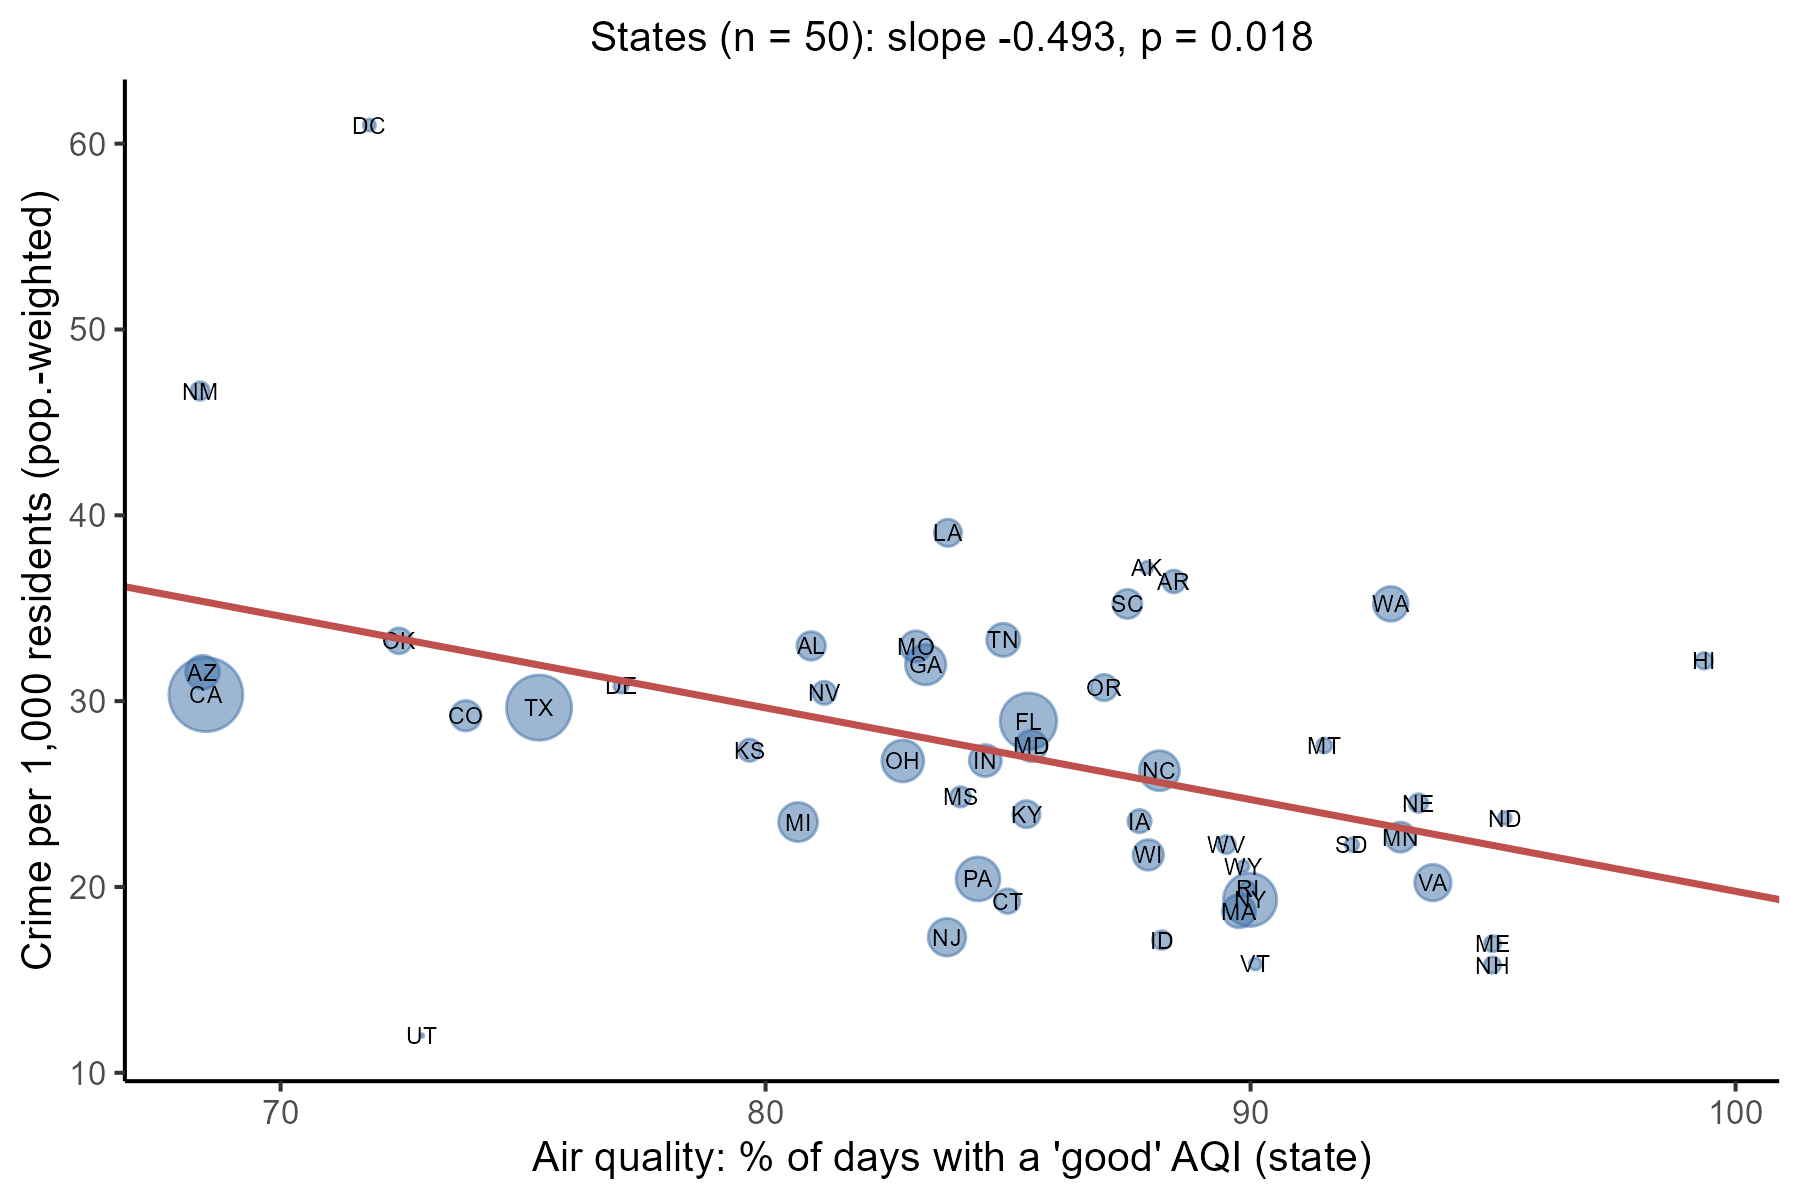
\includegraphics[width=\linewidth]{fig_state_aqi.png}
\caption{Crime vs.\ air quality across states (population-weighted; point size =
population). Low good-air states cluster in the West.}
\end{minipage}\hfill
\begin{minipage}[t]{0.49\textwidth}
\centering
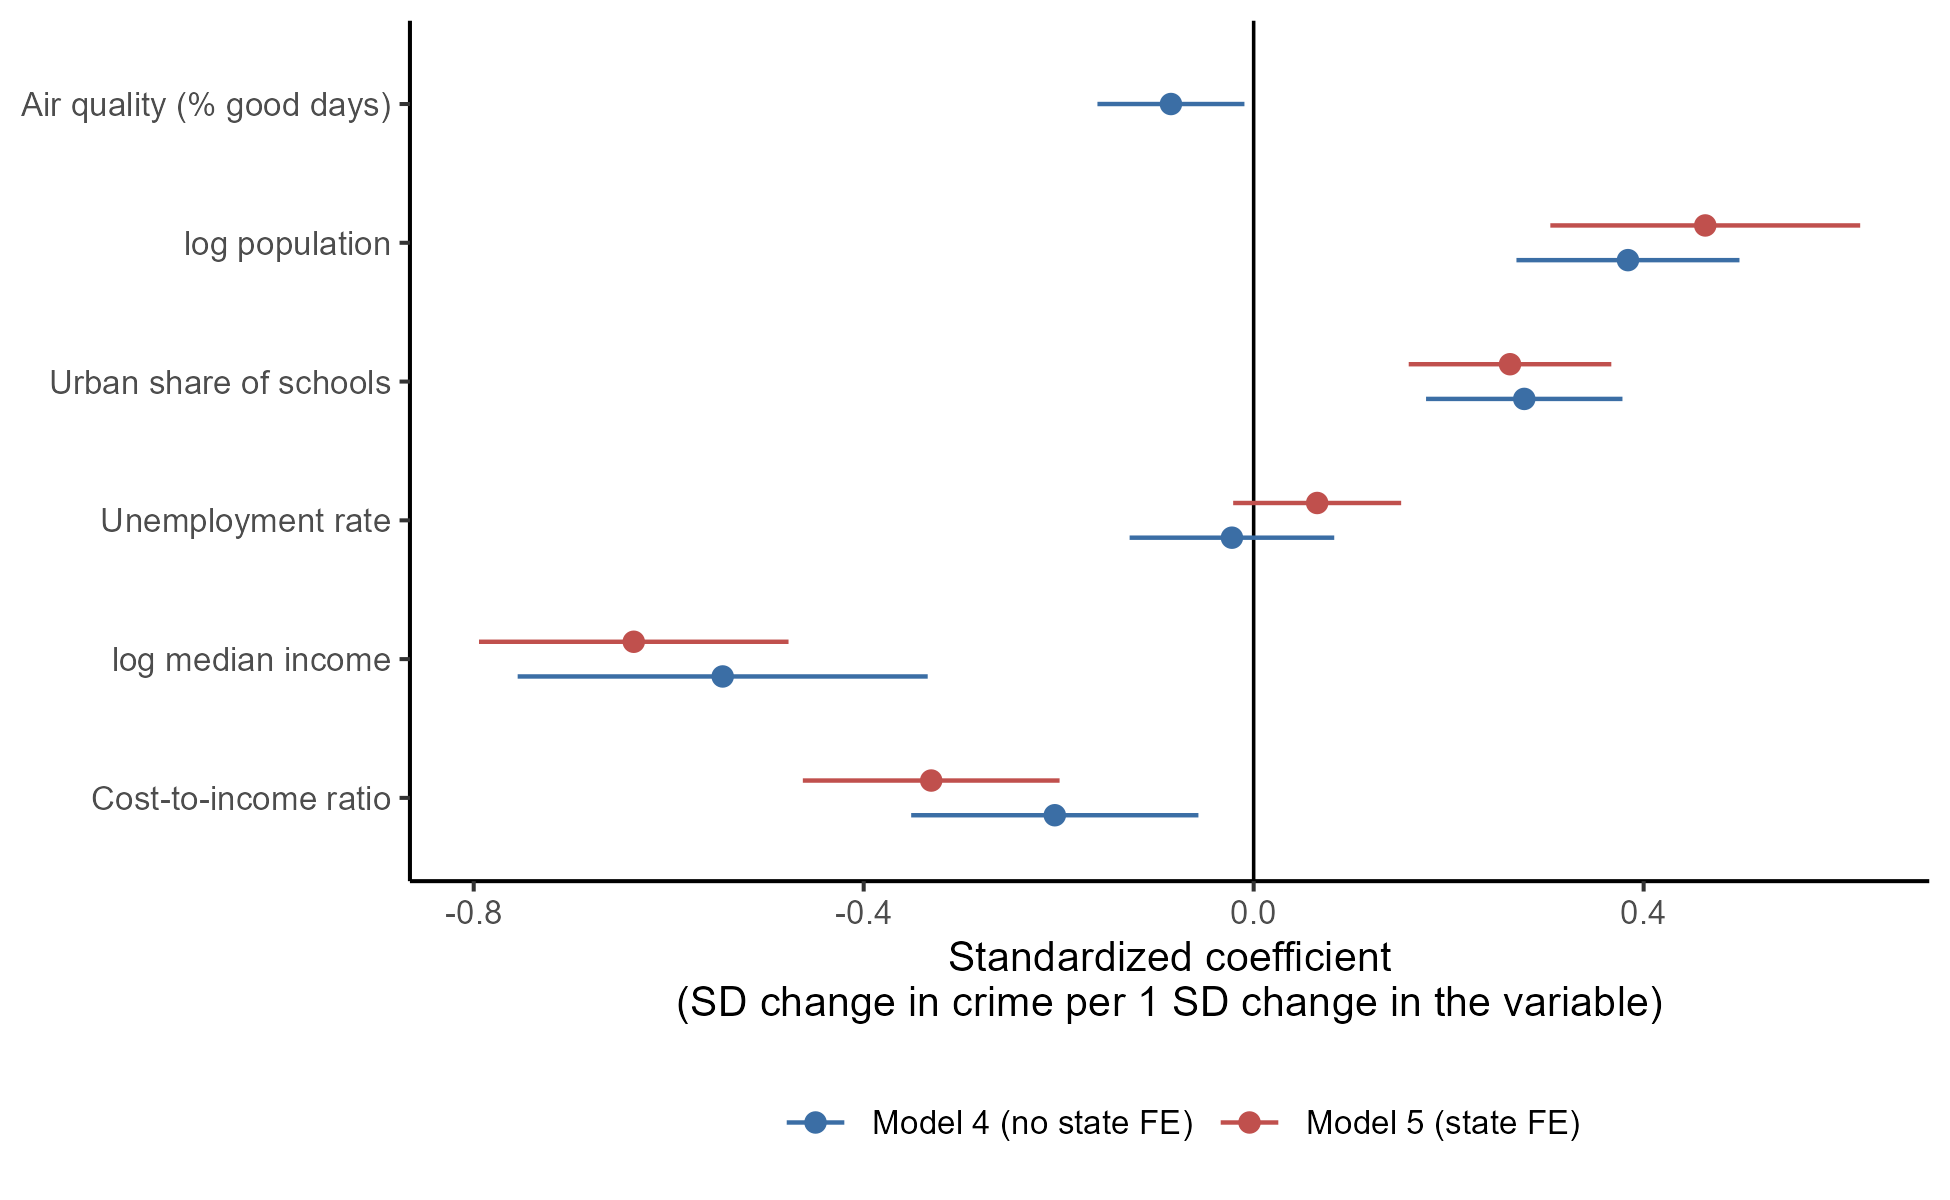
\includegraphics[width=\linewidth]{fig_std_coefs.png}
\caption{Standardized coefficients with 95\% CIs; Model 5 compares counties within a state
(air quality drops out).}
\end{minipage}
\end{figure}

\begin{table}[H]
\centering
\caption{The air-quality slope (crimes per 1,000 per percentage point of good-air days) as
the analysis is corrected step by step.}
\small
\begin{tabular}{@{}llccc@{}}
\toprule
Step & Specification & Slope & SE & $p$ \\
\midrule
0 & School rows, conventional SE (first version) & $-0.369$ & 0.005 & $<10^{-16}$ \\
1 & Counties, SE clustered by state & $-0.303$ & 0.085 & $<0.001$ \\
2 & + population, urbanization, income, unemployment, cost-to-income & $-0.154$ & 0.068 & 0.028 \\
3 & + Census region fixed effects & $-0.063$ & 0.069 & 0.365 \\
4 & + Census division fixed effects (instead of regions) & $-0.051$ & 0.072 & 0.488 \\
\bottomrule
\end{tabular}
\end{table}

\section{Conclusions}
Income and urbanization, not cost of living or state-level air quality, are the features most
strongly associated with county crime. The result does not contradict studies finding that
short-run pollution spikes raise violent crime \cite{bondy2020}; a state average is too
coarse to detect such effects. Methodologically, the project shows three common ways a
``significant'' result can be spurious: repeating group-level values across rows
\cite{moulton1990,cameron2015}, confounders that offset each other, and an area-level
variable that proxies for geography. A county-year panel with satellite PM$_{2.5}$ and
violent-crime data would be the natural next step.

\vspace{-4pt}
{\footnotesize
\renewcommand{\refname}{\normalsize References}
\begin{thebibliography}{9}\setlength{\itemsep}{0pt}
\bibitem{glaeser1999} Glaeser, E.\,L., \& Sacerdote, B. (1999). Why is there more crime in
cities? \textit{Journal of Political Economy}, 107(S6), S225--S258.
\bibitem{sampson1997} Sampson, R.\,J., Raudenbush, S.\,W., \& Earls, F. (1997).
Neighborhoods and violent crime. \textit{Science}, 277(5328), 918--924.
\bibitem{bondy2020} Bondy, M., Roth, S., \& Sager, L. (2020). Crime is in the air.
\textit{Journal of the Association of Environmental and Resource Economists}, 7(3), 555--585.
\bibitem{reyes2007} Reyes, J.\,W. (2007). Environmental policy as social policy? \textit{The
B.E. Journal of Economic Analysis \& Policy}, 7(1).
\bibitem{vaughan} Zac Vaughan. City/ZIP/County/FIPS -- Quality of Life (US). Kaggle.
\url{https://www.kaggle.com/datasets/zacvaughan/cityzipcountyfips-quality-of-life}.
\bibitem{moulton1990} Moulton, B.\,R. (1990). An illustration of a pitfall in estimating the
effects of aggregate variables on micro units. \textit{Review of Economics and Statistics},
72(2), 334--338.
\bibitem{cameron2015} Cameron, A.\,C., \& Miller, D.\,L. (2015). A practitioner's guide to
cluster-robust inference. \textit{Journal of Human Resources}, 50(2), 317--372.
\end{thebibliography}}

\end{document}
